\chapter{Metodologia}\label{cap_metodologia}

Nesse capítulo serão apresentados os passos metodológicos para abordar o problema proposto, que tem como objetivo principal
estudar a formação e consolidação de memórias em RNPs, com foco em analisar o impacto do sono nesse processo. Para estudar a
influência do sono na formação e recordação de assembleias neu\-ro\-nais foi proposto um modelo que simula uma RNP com diferentes
formas de plasticidade, baseado no trabalho de~\citeonline{zenkeDiverse2015}. A Figura~\ref{fig_metodologia} apresenta uma visão
geral da metodologia, contendo os passos para criação do modelo, que serão descritos nas seções subsequentes.

\begin{figure}[!ht]
\caption{Visão geral da metodologia: passos para construção do modelo e simulação e análise.}
\centering{
\parbox{12cm}{
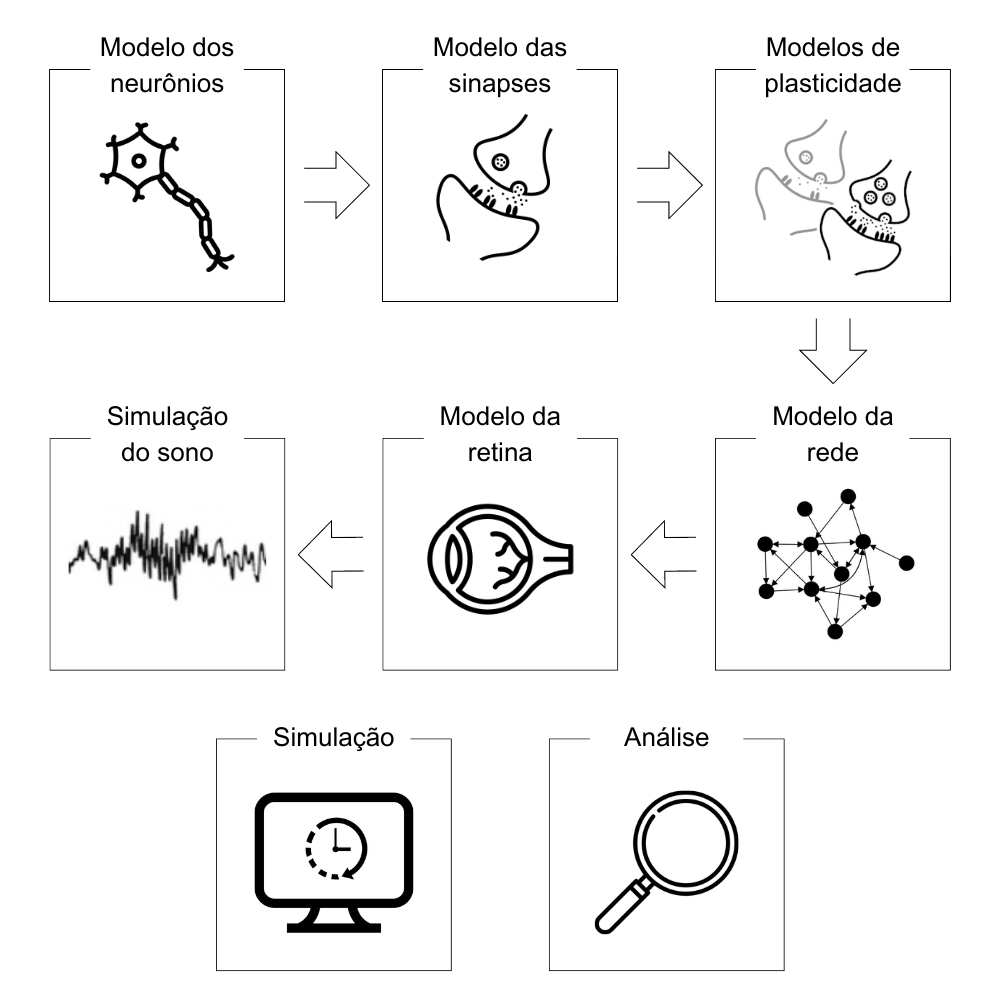
\includegraphics[width=12cm]{figuras/metodologia.png}\label{fig_metodologia}
\fonte{Elaborado pelo autor (2023).}
}}
\end{figure}


\section{Modelo dos neurônios}\label{sec_modelo_neuronios}

A unidade básica de uma RNP é o neurônio, então o primeiro passo para o modelo é a modelagem do neurônio. O modelo de neurônio
utilizado foi o \textit{Leaky Integrate-and-Fire} (LIF) devido à sua simplicidade, que captura o comportamento geral de um
neurônio enquanto permite simulações rápidas de larga escala, como apresentado na Seção~\ref{section_modelos_neuronios}.

O modelo LIF utilizado possui algumas diferenças do descrito na Seção~\ref{section_modelos_neuronios}, pois implementa adaptação
por frequência de disparo\footnote{Comportamento de um neurônio que reduz sua frequência de disparo em resposta a um estímulo
constante.} assim como o trabalho de~\cite{zenkeDiverse2015}, e apresentado na Equação~\ref{eq_lif_sfa}.

\begin{equation}
\label{eq_lif_sfa}
\tau^m\frac{d}{dt}v_i = (v^{rest} - v_i) + g_i^{exc}(t)(v^{exc} - v_i)+ (g_i^{gaba}(t) + g_i^{a}(t))(v^{ini} - v_i)
\end{equation}

\noindent{}onde $v_i(t)$, $v^{rest}$, $v^{exc}$, $v^{ini}$ se referem, respectivamente, ao potencial de membrana do neurônio,
potencial de repouso, potencial excitatório e potencial inibitório. As condutâncias são descritas por $g_i^{exc}(t)$,
$g_i^{gaba}(t)$, $g_i^{a}(t)$, respectivamente, excitatória, inibitória pelos neurônios pré-sinápticos GABAérgicos e inibitória
pela adaptação por frequência de disparo.

\section{Modelo das sinapses}\label{sec_modelo_sinapses}

Para simular como os neurônios interagem entre si, é preciso modelar as sinapses e como as condutâncias apresentadas na
Seção~\ref{sec_modelo_neuronios} evoluem com o tempo. Para isso, foi utilizado o modelo de sinapse de condução, apresentado na
Seção~\ref{subsection_modelos_sinapses}, mas com algumas diferenças notáveis. O comportamento das condutâncias inibitórias está
definido nas Equações~\ref{eq_lif_sfa_ini} e~\ref{eq_lif_sfa_a}:

\begin{equation}
\label{eq_lif_sfa_ini}
\frac{d}{dt}g_i^{gaba} = -\frac{g_i^{gaba}}{\tau^{gaba}} + \sum_{j\in ini}{w_{ij}S_j(t)}
\end{equation}

\begin{equation}
\label{eq_lif_sfa_a}
\frac{d}{dt}g_i^{a} = -\frac{g_i^{a}}{\tau^{a}} + \Delta^{a}S_i(t)
\end{equation}

\begin{equation}
\label{eq_lif_sfa_spikes}
S_j(t) = \sum_{k}{\delta(t-t_j^k)}
\end{equation}

\noindent{}onde $w_{ij}$ refere-se ao peso da sinapse do neurônio $i$ para o $j$. A Equação~\ref{eq_lif_sfa_spikes} representa a
soma de disparos no momento $t$. Nessas equações, a condutância $g$ tende a zero com o tempo, mas quando há um disparo dos
neurônios pré-sinápticos essa condutância sobe, exceto no caso da condutância pela adaptação do neurônio, que aumenta seguindo um
fator $\Delta^{a}S_i(t)$ quando o próprio neurônio dispara.

As sinapses excitatórias são modeladas com um componente rápido AMPA\footnote{ácido $\alpha$-amino-3-hidroxi-5-metil-4-isoxazol
propiônico} $g_i^{ampa}$ e um componente NMDA\footnote{N-metil-D-aspartato} $g_i^{nmda}$ que aumenta e decai lentamente, como
detalhado nas Equações~\ref{eq_lif_sfa_exc},~\ref{eq_lif_sfa_ampa} e~\ref{eq_lif_sfa_nmda}:

\begin{equation}
\label{eq_lif_sfa_exc}
g_i^{exc}(t) = \alpha g_i^{ampa}(t) + (1-\alpha)g_i^{nmda}(t)
\end{equation}

\begin{equation}
\label{eq_lif_sfa_ampa}
\frac{d}{dt}g_i^{ampa} = -\frac{g_i^{ampa}}{\tau^{ampa}} + \sum_{j\in exc}{w_{ij} 
\underbrace{u_j(t)x_j(t)}_{\text{PCP}}
S_j(t)}
\end{equation}

\begin{equation}
\label{eq_lif_sfa_nmda}
\tau^{nmda} \frac{d}{dt}g_i^{nmda} = -g_i^{nmda} + g_i^{ampa}
\end{equation}

As conexões excitatórias da RNP também têm a Plasticidade de Curto-Prazo (PCP) simulada pelas variáveis $u_j(t)$ e $x_j(t)$.

Quando $v_i$ utltrapassa seu limiar $\vartheta_i$, o potencial retorna para seu potencial de membrana $v_i^{rest}$. Quando há um
disparo, o limiar aumenta $\vartheta_i \rightarrow \vartheta^{disparo}$ para implementar o período refratário do neurônio, mas na
ausência de disparos, ele retorna lentamente a seu valor usual, como demonstra a Equação~\ref{eq_lif_sfa_thr}:

\begin{equation}
\label{eq_lif_sfa_thr}
\tau^{th}\frac{d\vartheta_i}{dt} = \vartheta^{rest} - \vartheta_i
\end{equation}


\section{Modelos de plasticidade}

As sinapses não são estáticas e têm diversas formas de plasticidade simuladas. As sinapses excitatórias implementam os seguintes
modelos de plasticidade: PCP, PDTD, heterossináptica e a induzida por transmissor, como apresentados na
Seção~\ref{section_modelos_plasticidade}.


\subsection{Plasticidade de curto-prazo}

Como apresentado na Seção~\label{sec_modelo_sinapses}, as variáveis $u_j(t)$ e $x_j(t)$ controlam a PCP, e suas dinâmicas estão
descritas nas Equações~\ref{eq_x} e~\ref{eq_u}:

\begin{equation}
\label{eq_x}
\frac{d}{dt} x_j(t) = \frac{1 - x_j(t)}{\tau^d} - u_j(t) x_j(t) S_j(t)
\end{equation}

\begin{equation}
\label{eq_u}
\frac{d}{dt}u_j(t) = \frac{U - u_j(t)}{\tau^f} + U(1 - u_j(t)) S_j(t)
\end{equation}

A Equação~\ref{eq_x} descreve a evolução da fração de recursos sinápticos disponíveis $x_j(t)$ ao longo do tempo, considerando
tanto a liberação quanto a recuperação de neurotransmissores. A Equação~\ref{eq_u} representa a variação na utilização desses
recursos $u_j(t)$ com o tempo, refletindo a probabilidade de liberação de neurotransmissores em resposta a um estímulo. Novamente,
$S_j(t)$ indica a presença de um disparo pré-sináptico, enquanto $\tau^d$ e $\tau^f$ são constantes de tempo que determinam a
velocidade de recuperação e decaimento dos recursos e da sua utilização, respectivamente. O termo $U$ representa a probabilidade
básica de liberação de um neurotransmissor em resposta a um único disparo.


\subsection{Plasticidade de longo-prazo}

Três tipos de plasticidade de longo-prazo afetam as sinapses excitatórias: PDTD $\mathfrak{P}(t)$ e  $\mathfrak{D}(t)$,
heterossináptica $\mathfrak{H}(t)$ e induzida por transmissor $\mathfrak{T}(t)$. Essas formas de plasticidade afetam diretamente o
peso da sinapse $w_{ij}$, como indica a Equação~\ref{eq_pdtd}:

\begin{samepage}

\begin{equation}
\label{eq_pdtd}
\frac{d}{dt}w_{ij}(t) = \mathfrak{P}(t) + \mathfrak{D}(t) + \mathfrak{H}(t) + \mathfrak{T}(t)\\
\end{equation}

\begin{align}
\begin{split}\label{eq_p}
  \mathfrak{P}(t) = Az_j^+(t) z_i^{lento}(t - \epsilon)S_j(t){} & \quad\quad\text{PLP tripla}
\end{split}\\
\begin{split}\label{eq_d}
  \mathfrak{D}(t) = - B_i(t)z_i^- (t)S_j(t){} & \quad\quad\text{DLP dupla}
\end{split}\\
\begin{split}\label{eq_h}
  \mathfrak{H}(t) = - \beta (w_{ij} - \bar{w}_{ij}(t)) (z_i^- (t - \epsilon))^3 S_i(t){} & \quad\quad\text{Heterossináptica}
\end{split}\\
\begin{split}\label{eq_t}
  \mathfrak{T}(t) = \delta S_j(t){} & \quad\quad\text{Induzida por transmissor}
\end{split}
\end{align}

\end{samepage}

As Equações~\ref{eq_p} e~\ref{eq_d} representam a potenciação e a depressão de longo-prazo, respectivamente, usando uma regra
tripla, ou seja, que leva em consideração 3 disparos~\cite{pfisterTriplets2006}. A Equação~\ref{eq_h} diz respeito à plasticidade
heterossináptica, ou seja, depende apenas do estado do neurônio pós-sináptico. A Equação~\ref{eq_t} implementa a plasticidade
induzida por transmissor, aquela que não depende no estado de nenhum neurônio, mas apenas na quantidade de transmissor presente.
Os parâmetros $A$, $\beta$ e $\delta$ são apenas escalares fixos, assim como $B_i(t)=A$. A variável $z_k^x(t)$ representa os
traços sinápticos dos neurônios pré- (índice $j$) e pós-sinápticos (índice $i$), e ela evolui de acordo com a Equação~\ref{eq_z}:

\begin{equation}
\label{eq_z}
\frac{d}{dt}z_i^x(t) = - \frac{z^x}{\tau^x}+S_i(t)
\end{equation}

\noindent{}em que $x$ pode tomar diferentes valores representando diferentes traços sinápticos. As variáveis $z^+$ e $z^-$
representam traços de atividade neuronal associados à potenciação e depressão sináptica, respectivamente. Quando um neurônio
pré-sináptico dispara antes de um pós-sináptico, isso pode levar ao aumento da força sináptica, relacionado ao traço $z^+$.
Inversamente, se o neurônio pós-sináptico dispara antes, a força sináptica pode diminuir, associado ao traço $z^+$. Já $z^{lento}$
refere-se a um traço que decai lentamente, capturando a atividade neuronal ao longo de um período de tempo mais extenso.

\subsubsection{Plasticidade de longo-prazo em sinapses inibitórias}

Também seguindo o modelo de~\citeonline{zenkeDiverse2015}, as sinapses inibitórias são moduladas pela PDTD hipotética descrita na
Equação~\ref{eq_pdtd_ini}, que basicamente tende a potencializar as sinapses inibitórias quando a atividade excitatória global da
rede estiver muito alta: 

\begin{equation}
\label{eq_pdtd_ini}
\frac{d}{dt}w_{ij}(t) = \eta G(t) [(z_i(t) + 1) S_j(t) + z_j(t) S_i(t)]
\end{equation}

\noindent{}onde $\eta$ é uma constante, $z_k$ representa os traços sinápticos e $G(t) = H(t) - \gamma$, em que $H(t)$ é o fator
global secretado, um valor que comprime toda a atividade do grupo excitatório e evolui segundo a Equação~\ref{eq_pdtd_ini_h}:

\begin{equation}
\label{eq_pdtd_ini_h}
\frac{d}{dt}H(t) = - \frac{H(t)}{\tau^H} + \sum_{i \in \text{exc}} S_i(t)
\end{equation}

Quando a atividade global da população excitatória $H(t)$ cai abaixo de um valor-alvo $\gamma$, $G(t)$ é menor que zero e a regra
de aprendizagem da Equação~\ref{eq_pdtd_ini} se torna uma regra unidirecional de ``depressão''. Se a atividade da rede for maior que
$\gamma$, a regra de aprendizagem se torna hebbiana. Isso serve para estabilizar a dinâmica geral da rede.

\section{Arquitetura da rede}

A rede é estruturada com um total de 5.120 neurônios do tipo LIF, distribuídos em dois grupos principais. O primeiro grupo é
formado por 4.096 neurônios excitatórios, enquanto o segundo grupo contém 1.024 neurônios inibitórios. Além disso, há grupos
auxiliares como a retina (Detalhada na Seção~\ref{subsection_retina}) e o grupo responsável pelos padrões de sono (Detalhado na
Seção~\ref{subsection_sono}). Para as conexões entre o grupo excitatório e inibitório, cada neurônio é conectado a 10\% dos
neurônios de outro grupo ou do seu próprio grupo, e essa conectividade é estabelecida de forma aleatória. As conexões excitatórias
entre neurônios são moduladas pelo neurotransmissor glutamato, com receptores AMPA e NMDA, enquanto as conexões inibitórias são
moduladas pelo neurotransmissor GABA.\@

\subsection{Modelo da retina}\label{subsection_retina}

De modo a simular a entrada de estímulos visuais, foi proposto um simulador para a retina, que é composta de 4.096 neurônios LIF,
com cada neurônio representando um pixel em uma imagem de 64$\times$64 pixels. Cada neurônio excitatório da RNP recebe conexões
dos neurônios da retina de uma área circular de raio 8, em que o centro do círculo é escolhido aleatoriamente para cada neurônio,
como exemplifica a Figura~\ref{fig_estimulo_raio}. As conexões da retina com a RNP também são plásticas.

\begin{figure}[!ht]
\caption{Exemplo de estímulo apresentado à RNP.\@ Aqui, um neurônio com seu campo receptivo centralizado no X recebe conexões dos neurônios da retina contidos dentro da grade verde.}
\centering{
\parbox{6cm}{

\includegraphics[width=6cm]{figuras/estimulo_raio.png}\label{fig_estimulo_raio}
\fonte{Elaborado pelo autor (2023).}}}
\end{figure}

No Capítulo~\ref{cap_experimentos}, será melhor detalhado quais os estímulos propostos para os experimentos, mas eles consistem em
imagens simples de serem reconhecidas, como formas geométricas e símbolos. Essas imagens são binárias: apenas preto e branco; o
neurônio da retina correspondente a um pixel preto dispara com frequência média de 10Hz, enquanto o neurônio correspondente a um
pixel branco dispara com frequência média de 35Hz, ou seja, com uma maior ativação.

\subsection{Simulação do sono}\label{subsection_sono}

Para simular o sono, a rede funciona de dois modos diferentes intercalados: um modo de atividade ou vigília, em que a rede
funciona normalmente enquanto recebe estímulos, e um modo de inatividade ou sono, em que será simulado o sono. 

Durante o ciclo de sono, nenhum estímulo é apresentado à rede, contudo, ela continua sendo simulada normalmente. Essa etapa é
subdividida em duas fases, correspondentes às fases do sono real: REM e NREM.\@ Em um ciclo completo de sono, as fases REM e NREM
se alternam, iniciando-se com a fase NREM, seguida pela REM, sendo que cada uma destas fases ocupa um oitavo da duração total do
sono. Assim, o ciclo de NREM e REM se repete quatro vezes em um ciclo completo de sono, de maneira análoga ao que ocorre nos
humanos, nos quais cada noite de sono compreende entre 4 a 6 ciclos~\cite{patelPhysiology2023}.

Para simular cada fase do sono, é utilizado um grupo de 256 neurônios excitatórios que se ativam de maneira sinusoidal e
conectam-se a 20\% dos neurônios do grupo de neurônios excitatórios. Durante a fase NREM, a frequência dessa onda de ativação
sinusoidal é de 1Hz, enquanto na fase REM é de 16Hz, visando aproximar-se, de forma simplificada, das frequências observadas
durante essas fases em humanos~\cite{guoSlow2022, cowdinTheta2014}. Este método foi inspirado no trabalho de~\citeonline{bazhenovModel2002}, que
simulou o sono de maneira similar, utilizando um grupo de neurônios com 25\% de conectividade com a rede, com um disparo médio de
25Hz modulados por uma função sinusoidal.

\subsection{Análise de assembleias neuronais}

A fase final do trabalho consiste em analisar as diferentes simulações realizadas e determinar se a simulação de sono teve algum
efeito na formação de assembleias neuronais. Para isso, antes de tudo é necessário definir um modo de identificar as assembleias
neuronais e quais neurônios pertencem a cada uma.

Para determinar quais neurônios pertencem à assembleia neuronal associada a um estímulo, o método consiste em analisar a
frequência de disparos de cada neurônio no intervalo $3s < t < 3.5s$ após a apresentação do estímulo. Os neurônios que disparam
com frequência maior que 20Hz nesse intervalo são considerados como pertencentes à assembleia neuronal associada a esse estímulo.
No trabalho de~\citeonline{zenkeDiverse2015} foram analisados os neurônios com frequência de disparos maior que 10Hz, mas nesse
trabalho optou-se por considerar apenas os com frequência maior que 20Hz, pois com esse valor a soma total de todos os neurônios
em assembleias neuronais chegou mais próximo do número total de neurônios da rede, incluindo neurônios repetidos em cada
assembleia.

\chapter{Experimentos}\label{section_experimento}

Como forma de avaliar o modelo proposto serão conduzidos dois principais experimentos.

\section{Experimento 1: Formação de assembleias neuronais}

O primeiro experimento consiste em simular a RNP apresentando estímulos ao modelo de retina e analisar se a repetição dos
estímulos leva à formação de assembleias neuronais associadas a cada estímulo a longo prazo, com o objetivo de ter uma base de
comparação para o experimento 2, que terá o sono simulado. Os estímulos consistem em seis imagens simples de serem reconhecidas,
exibidas na Figura~\ref{fig_estimulos}, e são apresentados à rede de forma intercalada e aleatória. Quatro estímulos foram
reaproveitados do trabalho de~\citeonline{zenkeDiverse2015}, enquanto as figuras de diamante e de cruz foram adicionadas com o
intuito de colocar a RNP mais próxima do seu limite.

\begin{figure}[!ht]
\caption{Os seis estímulos apresentados à RNP durante os experimentos.}
\centering{
\parbox{12cm}{
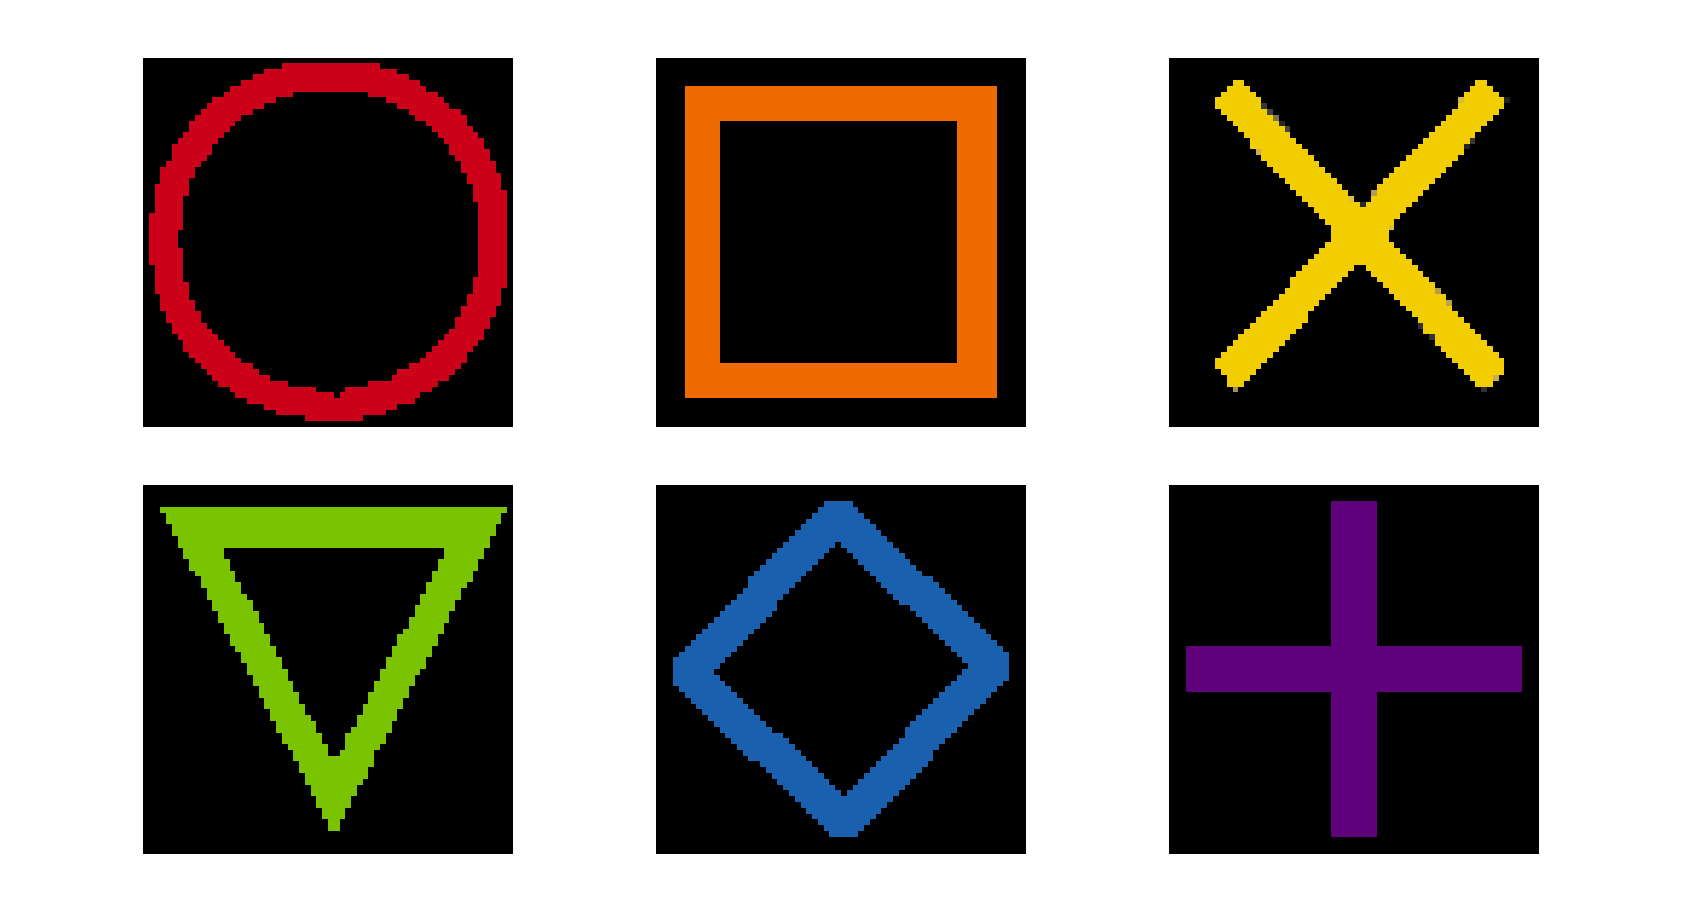
\includegraphics[width=12cm]{figuras/estimulos_cor.png}\label{fig_estimulos}
\fonte{Elaborado pelo autor (2023).}}}
\end{figure}

Houveram três fases da simulação da RNP:

\begin{enumerate}
  \item Simulação da rede em seu estado inicial por 1800 segundos, com um tempo médio de aparição do estímulo de 2 segundos, e
  tempo médio entre estímulos de 1 segundo. O peso das sinapses entre a retina e a rede é de 0.05.
  \item Simulação da rede também por 1800 segundos, mas com um tempo médio de aparição do estímulo de 0.2 segundo, e
  tempo médio entre estímulos de 5 segundos. O peso das sinapses entre a retina e a rede agora é de 0.1. A intenção aqui é
  fazer com que a rede tenha mais tempo entre um estímulo e outro para poder memorizá-los melhor.
  \item A última simulação é de 2400 segundos e é de onde são tirados os resultados. O tempo médio de aparição do estímulo diminui
  para 0.1, enquanto o tempo médio entre estímulos é de 10 segundos, com a intenção de ter uma janela maior de tempo entre os
  estímulos para analisar a capacidade de memorização da RNP.
\end{enumerate}


\section{Experimento 2: Formação de assembleias neuronais com sono}

De forma similar ao experimento 1, o segundo experimento consiste em simular a RNP apresentando os mesmos estímulos, mas dessa vez
com a simulação de sono. O objetivo desse experimento é analisar se a simulação de sono tem algum efeito na formação de
assembleias neuronais.

Esse experimento seguiu as mesmas três fases do experimento anterior, mas com a simulação do sono. Nesse experimento, a RNP ficava
em estado de vigília por 200s e dormia por 100s, seguindo uma proporção similar a de humanos que ficam acordados 16 horas por dia
e dormem 8~\cite{waterhouseDaily2012}.

\section{Análise dos resultados}

\subsection{Formação de assembleias neuronais}

O número médio de neurônios por assembleia neuronal na RNP base foi de 787, enquanto na RNP com sono foi de 432.67; isso se deve
principalmente ao fato de que as assembleias neuronais do círculo e do quadrado tiveram pouquíssimos neurônios, apenas 42 e 34 na
RNP com sono. Ambas as RNPs tiveram dificuldades em manter uma assembleia neuronal única para o estímulo do círculo, havendo
bastante sobreposição com os neurônios da assembleia neuronal do quadrado; isso provavelmente ocorre pela similaridade entre os
dois estímulos e também a possibilidade da RNP ter alcançado um limite de memória. A matriz de sobreposição das assembleias
neuronais está ilustrada nas Figura~\ref{fig_mat_base}.

\begin{figure}[!ht]
\caption{Matrizes contendo o número de neurônios pertecentes a cada assembleia neuronal. Os elementos da diagonal principal da
matriz indicam o número total de neurônios em cada assembleia individual. Nos outros casos, o elemento representa quantos
neurônios de uma assembleia também são parte de outra assembleia.}

\centering{
\parbox{\linewidth}{
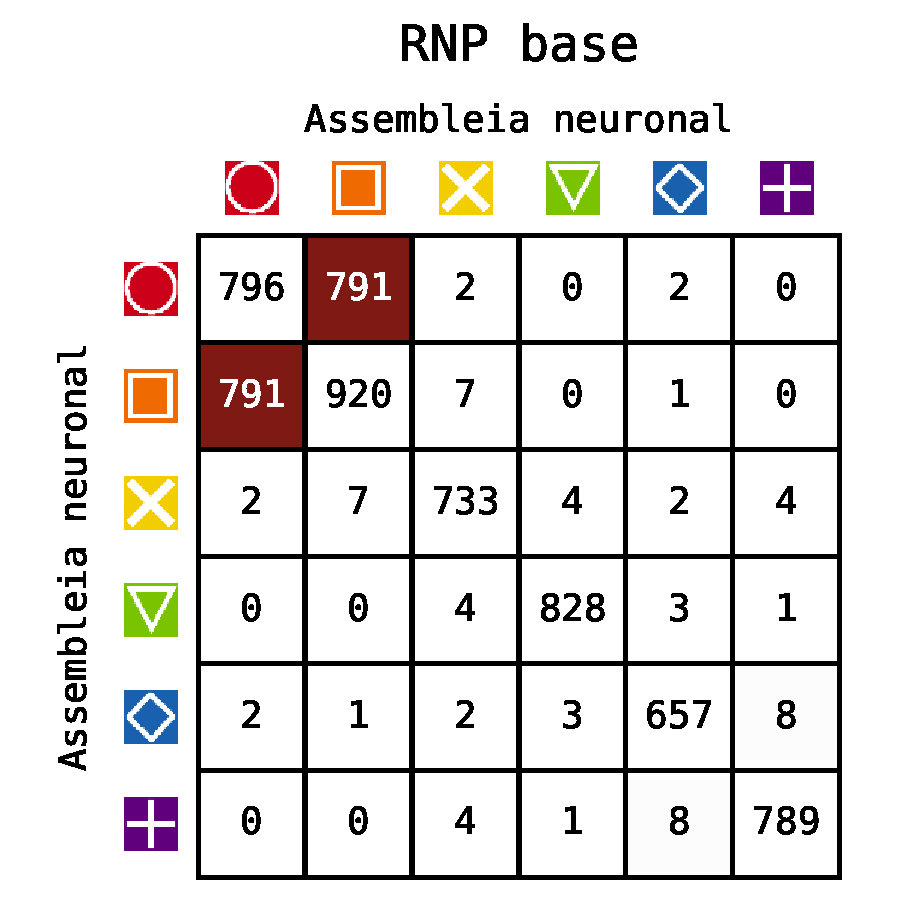
\includegraphics[width=7.5cm]{figuras/plots_pdf/RNP base.pdf}\label{fig_mat_base}
\hfill
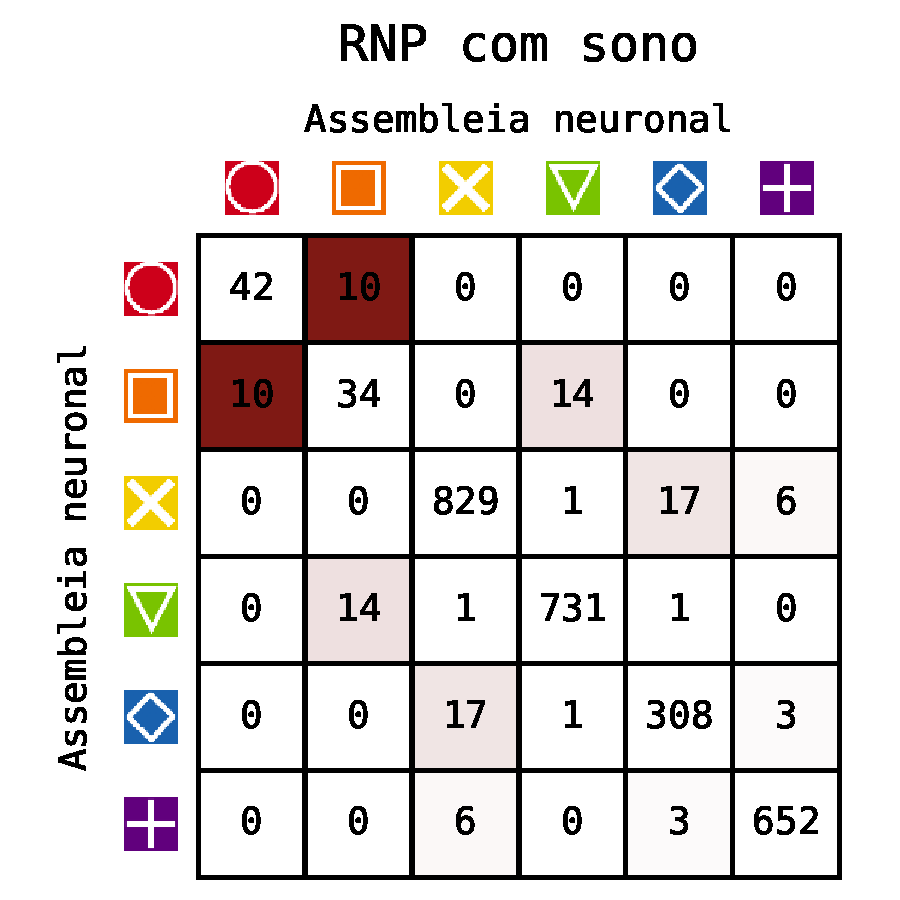
\includegraphics[width=7.5cm]{figuras/plots_pdf/RNP com sono.pdf}\label{fig_mat_sleep}
\fonte{Elaborado pelo autor (2023).}}}
\end{figure}

Outra forma de analisar o comportamento das RNPs é verificando a ativação média das assembleias neuronais para cada estímulo, como
mostra a Figura~\ref{fig_mat_act_base}. A diagonal principal claramente possui as maiores médias pois a assembleia neuronal de um
determinado estímulo vai apresentar muito mais atividade para esse estímulo. Nota-se também que na RNP com sono houve mais
atividade nas assembleias neuronais não relacionadas com o estímulo, indicando uma piora na performance.

\begin{figure}[!ht]
\caption{Matrizes representando a ativação média em Hz de cada assembleia neuronal para cada estímulo diferente.}
\centering{
\parbox{\linewidth}{
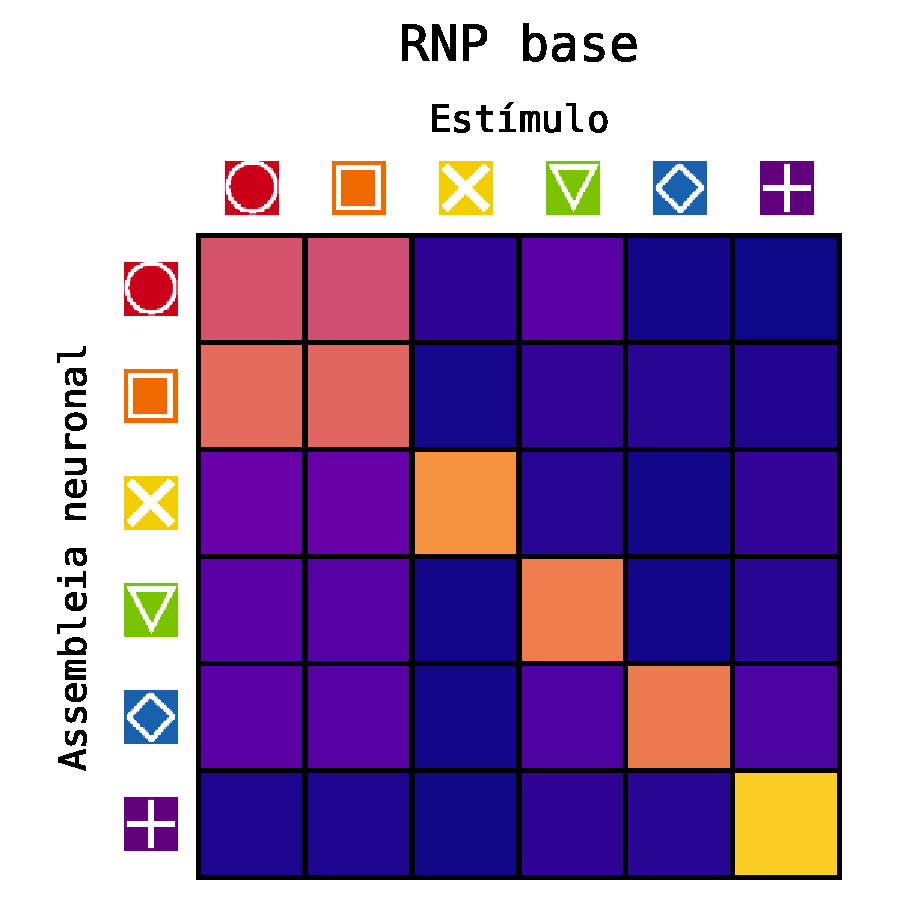
\includegraphics[height=7cm]{figuras/plots_pdf/RNP base_atv.pdf}\label{fig_mat_act_base}
\hfill
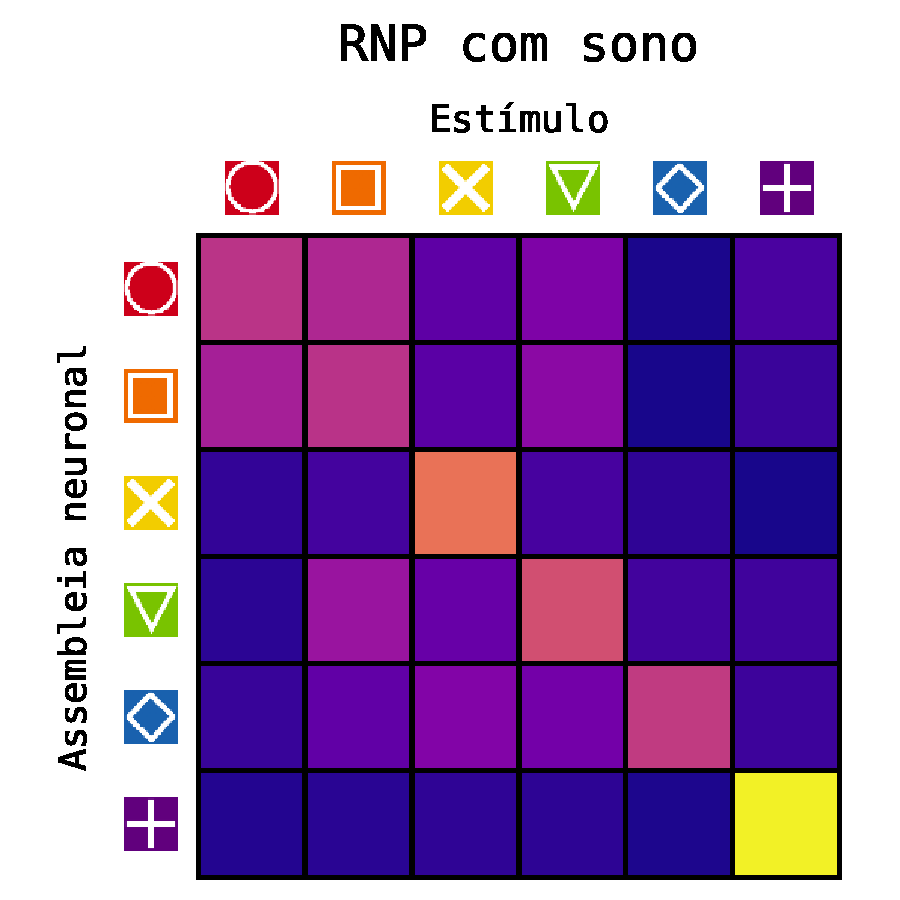
\includegraphics[height=7cm]{figuras/plots_pdf/RNP com sono_atv.pdf}\label{fig_mat_act_sono}
\hfill
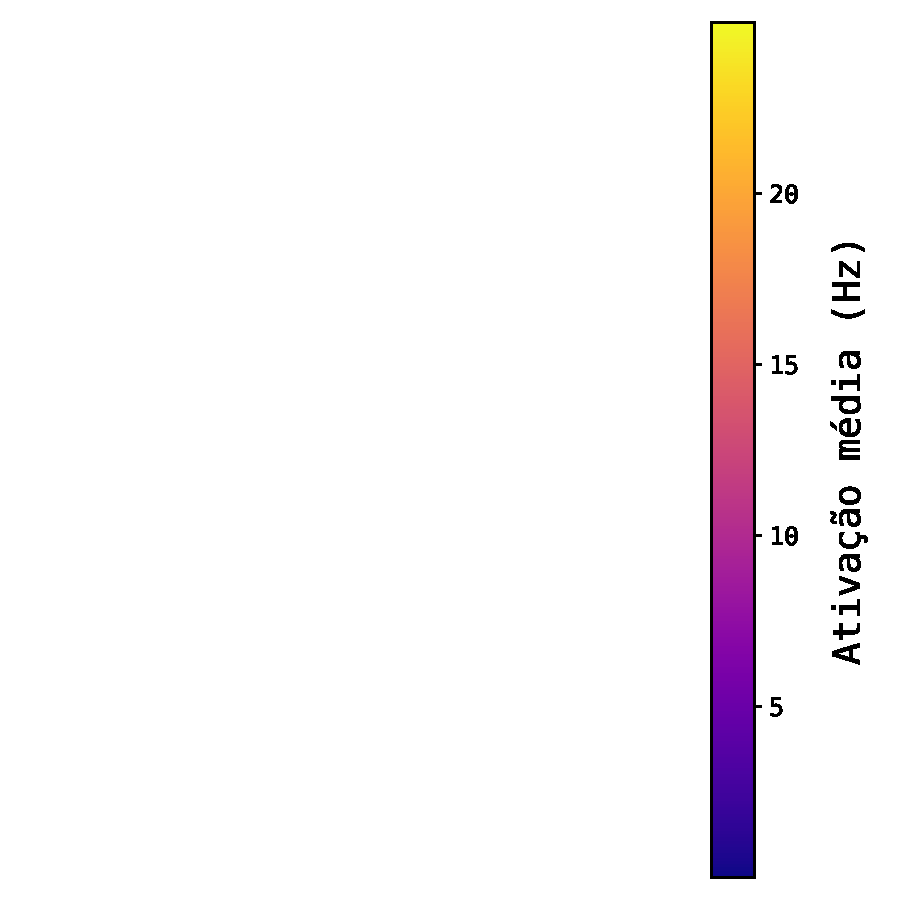
\includegraphics[height=5.8cm]{figuras/plots_pdf/atv_colorbar.pdf}\label{fig_mat_act_colorbar}
\fonte{Elaborado pelo autor (2023).}}}
\end{figure}

Com base nesses resultados, pode-se deduzir que a simulação do sono não afetou significativamente a formação de assembleias
neuronais, ou que no máximo serviu apenas para limitar as capacidades da rede.

\subsection{Atividade da RNP}

Outra forma de analisar os resultados da simulação é analisando diretamente os dados dos disparos dos neurônios. A
Figura~\ref{fig_base_act} contém um gráfico relacionando o momento dos estímulos (topo da figura) com a ativação média das
assembleias neuronais (parte inferior da figura). É possível identificar que na maioria das vezes em que um estímulo é apresentado
à RNP, a assembleia neuronal associada a esse estímulo dispara e mantém-se ativa até que outro estímulo domine a atividade da
RNP;\@é importante notar que o estímulo é mostrado para a RNP por menos de 1 segundo, portanto a ativação da assembleia neuronal
nos segundos seguintes é a memória do estímulo.

Também pode-se notar que quando é mostrado o estímulo do círculo ou do quadrado, as assembleias neuronais de ambos os estímulos
disparam juntas, devido à sobreposição de neurônios entre as duas assembleias neuronais\footnote{Se é que podem ser consideradas
duas assembleias neuronais, já que os neurônios são quase todos os mesmos em ambas.} identificada na seção anterior.

\begin{figure}[!ht]
\caption{Ativação das assembleias neuronais na simulação da RNP base.}
\centering{
\parbox{\linewidth}{
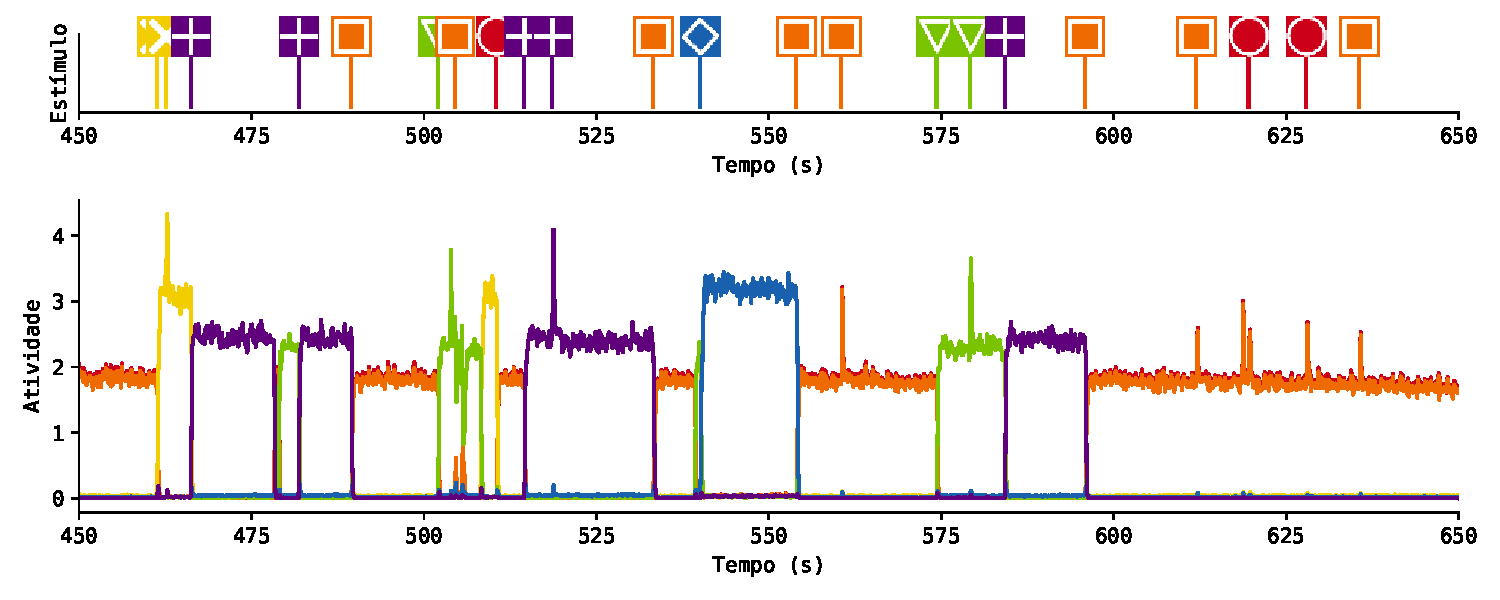
\includegraphics[width=\linewidth]{figuras/plots_pdf/atividade base.pdf}\label{fig_base_act}
\fonte{Elaborado pelo autor (2023).}}}
\end{figure}

Durante as simulações de sono da RNP, em diversas instâncias foram observados padrões intrigantes de atividade, como ilustrado nas
Figuras~\ref{fig_sleep_act} e~\ref{fig_sleep_act2}. Em várias casos, ao entrar no modo de sono, a RNP mantém uma atividade
consistente de uma assembleia neuronal, correspondente à resposta ao último estímulo mostrado a ela. Esta atividade é sustentada
por algum tempo, no entanto, há um momento em que ela diminui e é substituída por uma nova assembleia neuronal que emerge com uma
série de disparos. Como uma assembleia neuronal é a representação de uma memória na RNP, essa reativação da assembleia neuronal
representa um momento durante o sono em que a RNP se recorda de algum estímulo.

\begin{figure}[!ht]
\caption{Ativação das assembleias neuronais na simulação da RNP com sono em momento de ``sonho''. A cor cinza indica o período de sono.}
\centering{
\parbox{\linewidth}{
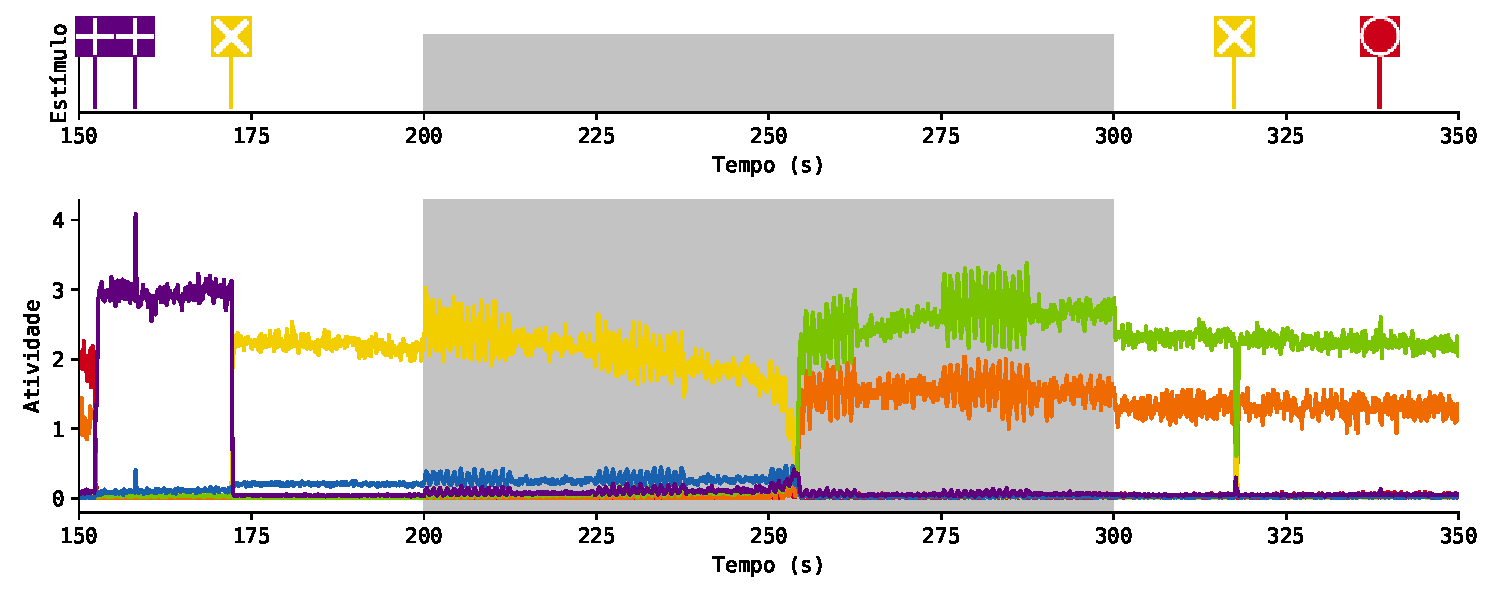
\includegraphics[width=\linewidth]{figuras/plots_pdf/atividade sonho1.pdf}\label{fig_sleep_act}
\fonte{Elaborado pelo autor (2023).}}}
\end{figure}

\begin{figure}[!ht]
\caption{Ativação das assembleias neuronais na simulação da RNP com sono em outro momento de ``sonho''. A cor cinza indica o período de sono.}
\centering{
\parbox{\linewidth}{
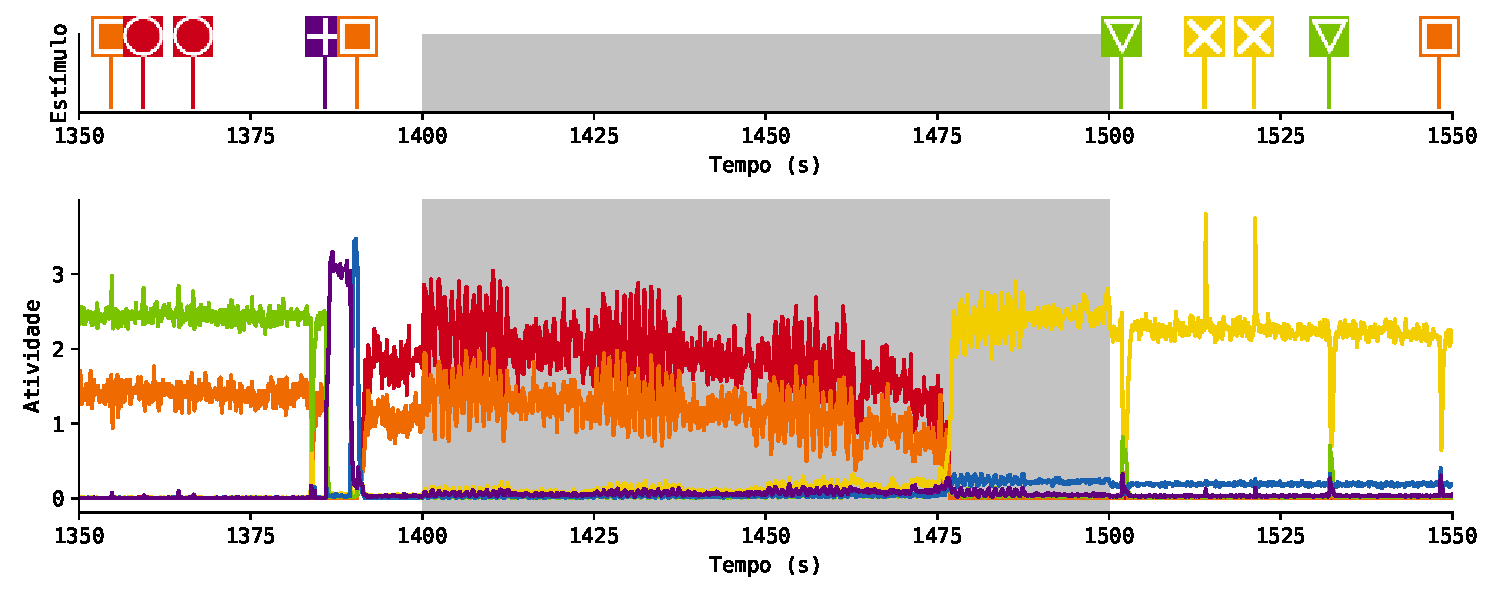
\includegraphics[width=\linewidth]{figuras/plots_pdf/atividade sonho2.pdf}\label{fig_sleep_act2}
\fonte{Elaborado pelo autor (2023).}}}
\end{figure}

Esse padrão de reativação da assembleia neuronal pode ser interpretado analogamente aos processos de sonho em organismos
biológicos. Segundo o trabalho de~\citeonline{picard-delandMemory2023}, existe um fenômeno observado durante o sono em que rastros
de memória recém-formados são reativados espontaneamente durante o sono, e esse fenômeno pode ou não estar conectado com a experiência de
sonhos e com a consolidação de memórias durante o sono.

No entanto, é fundamental abordar esta interpretação com cautela. Embora as semelhanças sejam intrigantes, é essencial
não tirar conclusões precipitadas e reconhecer que mais pesquisas são necessárias antes de afirmar que esses padrões representam
efetivamente ``sonhos'' em RNP.\@

